\paragraph{Current Approaches.}

% Consider an autonomous unmanned surface vehicle (USV) guarding a valuable asset in the ocean when an unknown vehicle  approaches the security perimeter, under challenging weather conditions. In this scenario, the USV is required to approach the intruding vehicle, issue a warning signal, and escort it to a safe distance from the controlled area. However, as the USV has no a priori knowledge of its external environment behaviors (e.g., water depth, waves, wind, current, visibility), pre-computing a feasible trajectory, let alone optimal, becomes a non-trivial problem. The USV must continuously sense a large set of parameters and update its estimations about the external world to compute a trajectory that is safe and satisfies the maneuverability constraints and the COLREGS rules. It must continuously generate traversability maps by sensing fixed and moving obstacles in the sensor range, by classifying moving obstacles, and by possibly predicting their trajectories.  
 
Over the last decade, machine learning (ML) algorithms have achieved impressive results in solving large-scale  perception problems for decision-making under uncertainty in cyber-physical systems (CPSs) (see, e.g.,~\cite{Blum97,Jia14,Michalski13}). 
% In our scenario, the USV may identify moving obstacles based on their physical appearance and motion signatures and generate traversability maps using ML classifiers; it may estimate the sensors' performance in adverse weather conditions and the uncertainty in the environment state using active learning; it may learn maneuvers that are compliant with the COLREGS   
% % Vessel behavior prediction based on motion histories 
% using reinforcement learning. 
% Learning pursuit behaviors using adversarial learning
While a successful mission will heavily depend on ML components, its safety-critical nature raises concerns on the overall system safety and trustworthiness. In fact, recent efforts toward the verification of ML programs~\cite{Szegedy2013} show how even well-trained neural networks can be sensitive to small perturbations, e.g., small modifications can lead the network to misclassify the altered input with large confidence. In systems with complex interactions, a misclassification error in one component may eventually compromise the entire mission.  
% We will need to make sure that each learning enabled components will have a run time monitor that will ensure that the assumptions made by the learning-enabled system remain valid and prevent erroneous learning.
% 
% For example, if the vehicle is exhibiting significant error in trajectory tracking, then simply downgrading the trajectory tracking error value may not be a good idea.  The failure of prediction of trajectory tracking error might be due to the presence of a significant wake caused by a nearby vessel.  The presence of the nearby vessel can be used as a conditional evidence to explain the poor trajectory tracking performance.
While exhaustive validation of learning-enabled cyber-physical systems (LE-CPSs) is a prohibitive task~\cite{Kalra16},
their complexity, heterogeneity, and highly dynamic nature
make it challenging to even leverage existing model-based development techniques to effectively assess  system correctness 
% dependability, 
and compliance with regulations at design time.
% In complex CPSs, the \emph{concept design phase} largely remains a manual process. Modern requirement-management tools are still predominantly centered on text-based languages, often not in the mother tongue of the engineer, which creates opportunities for ambiguities, redundancies, and potential conflicts~\cite{Feldman16}. During system development,  different design portions tend to use domain-specific languages and (DSLs) tools that are poorly inter-operable, which makes it hard to combine the results of different analysis or synthesis methods.    
% The complexity of the underlying ML algorithms, their large feature spaces, and the lack of consensus on a formal definition of correctness can only exacerbate these issues. 
LE-CPSs require significant levels of adaptiveness and resilience to unpredictable scenarios. 
% for example, in response to changes in the environment or in the operating conditions of the learning components with respect to their training conditions. 
For these systems, assumptions made at design time may break at run time, and correctness claims must often be  based on evidence that can only be provided during system operation.  
% and conventional frameworks are not able to capture adaptiveness under uncertain, faulty, or adversarial scenarios.

% Our approach
\emph{In this project, we address the LE-CPS design challenges via a holistic approach. 
% that can contextually generate design artifacts and assurance cases. 
Rather than focusing on ML components in isolation, we seek to systematically specify and analyze the behaviors of ML components within the context of a CPS. 
% We treat safety as an emergent property of the system, wherein unintended interactions and performance constraint violations are sometimes more consequential than failed components. 
We develop a modeling framework, methods, and tools to support the design process from system-level requirement capture, formalization, and analysis, to the generation, testing, and continual monitoring of software and hardware artifacts in feedback loop with a physical process.}
% coordinated research effort toward the development of (i) a novel compositional contract-based framework for LE-CPSs, (ii) theories and tools for cross-layer, resilient, LE-CPS design, including modeling and construction of high-assurance learning systems, and (iii) an all-encompassing methodology bridging design-time and dynamic assurance.

We will pursue a contract-based approach~\cite{Nuzzo15b,Sangiovanni-Vincentelli2012a} leveraging modularity and compositional reasoning to enhance the \emph{scalability} of design and verification tasks and aiming to produce artifacts that are \emph{correct-by-construction}. 
A contract can be intuitively seen as a pair $(A,G)$ of properties, where $A$ specifies the assumptions that a component makes on the external environment and $G$ the guarantees it provides under these assumptions. In contract-based design, formal support for assume-guarantee reasoning is directly built into the modeling framework since the early design stages. Contracts enable modular and hierarchical verification of global properties of a system, whose satisfaction can be proven based on the satisfaction of local properties of the components~\cite{Cimatti15b}. Contracts support stepwise refinement, where hierarchical specifications can be used to reason about component decompositions, even if the component implementations are not yet available~\cite{Cimatti15b,Nuzzo14,Iannopollo14}. Contracts facilitate component reuse, as any components satisfying a contract directly inherit its guarantees~\cite{Iannopollo14}. 
% 
% Contract constructs, carrying claims as well as evidence, context and assumptions, thus become critical reasoning elements in our dynamic assurance case.

Overall, contracts have shown to be effective for specifying and reasoning about systems, especially when component models belong to the same level of abstraction (e.g., algorithm, software, architecture) or adopt the same formalism. 
However, there is no universal modeling formalism that can capture every aspect of complex, heterogeneous LE-CPSs, and guarantee, at the same time, tractable analysis. Designers usually ``decompose'' a complex system into semantically different models, by adopting the most convenient formalisms to represent different design viewpoints (e.g., system functionality, timing, safety, and reliability) at different abstraction levels. They then leverage the most suitable tools to analyze and synthesize these models separately. 
For example, the control law for a vehicle is typically derived and initially evaluated using control-oriented models, e.g., discrete-time linear models, in which details of the implementation and the physical dynamics are simplified or neglected. These details are usually modeled and evaluated using other formalisms and tools, e.g., by simulation of continuous-time differential algebraic equations (DAE). Each model represents some aspects of system design and occludes others, by making simplifying assumptions that are often undocumented or informally captured at best. A set of challenges then remain for model-based design flows when models are to be formulated and manipulated along the design flow, across different abstraction levels, and between design time and operation time. ML components further exacerbate these difficulties due to the lack of practical and reliable abstractions that can encompass 
% including different algorithms and heterogeneous architectures, such as .  
the heterogeneity of ML algorithms and architectures (e.g., data-driven classifiers for perception and situational awareness, reinforcement learning for developing control policies, and algorithms for learning system dynamics) and the different nature of their performance and safety guarantees.  
% make it daunting to devise reliable  to guarantee the performance and correctness of the entire system. 

% While contract theories promise to encompass any kind of formalism and decomposition, it is not always clear how they can effectively support the correct transition between heterogeneous abstraction levels, and between design and operation time. 
% In fact, the notions of contract abstraction and refinement are traditionally defined in the context of a single formalism, e.g., using language inclusion or simulation relations. 


Our vision for LE-CPS design is that compositional abstractions should bridge heterogeneous formalisms and heterogeneous decomposition architectures, to make system analysis and synthesis tractable, to consistently combine different verification and synthesis methods at design time, and to provide seamless support for dynamic assurance at run time. This requires new abstraction mechanisms to quantitatively capture the confidence in the satisfaction of requirements under uncertain or unknown conditions, and resilience properties of  systems at both the abstract (algorithm) and the concrete (physical, hardware, and software) levels, to enable trade-off evaluation between resilience, performance, and cost. This vision informs the research efforts detailed below. 



\vspace{-.2in}\subsubsection{System Architecture and Design Approach}
\vspace{-.1in}


\begin{wrapfigure}{R}{0.5\textwidth}
\vspace{-30pt}
\begin{center}
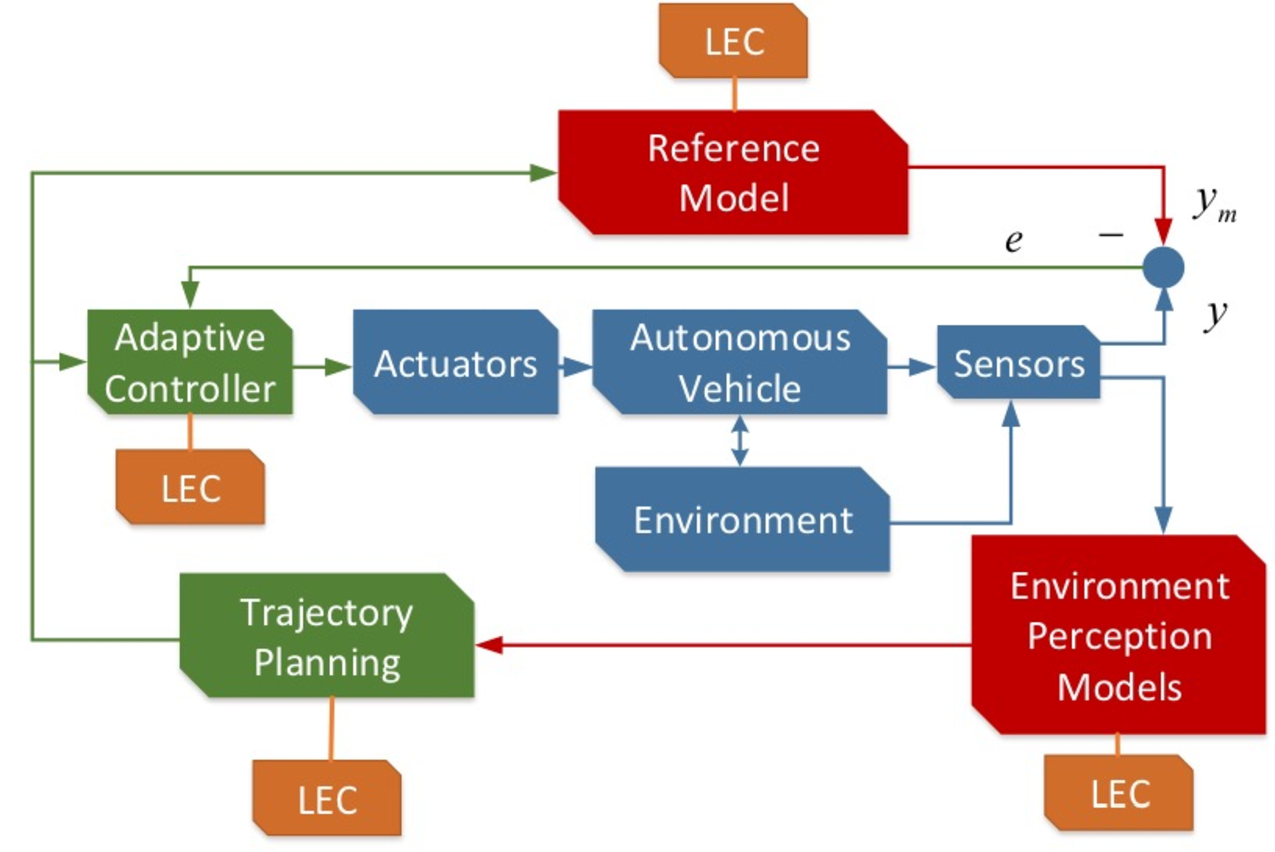
\includegraphics[width=0.5\textwidth,trim={0in 0.15in 0in 0in},clip]{./TA1/Architecture.pdf}
\caption{Simplified control architecture for a LE autonomous system.}
\label{fig:architecture}
\end{center}
\vspace{-25pt}
\end{wrapfigure}

% \textcolor{blue}{\begin{itemize}
% \item
% What is the baseline capability of the proposed methods, in terms of the hybrid state-space and number and complexity of learning-enabled components?
% \item
% How do you plan to scale up by an order of magnitude?
% \item
% How will you characterize the tradeoffs between fidelity of your modeling
% abstractions and scalability of the verification approach.
% \item
% What is the baseline overhead of the operation-time assurance monitoring
% techniques?
% \item
% How do you plan to minimize it to be below 10\% of the nominal system resource utilization?
% \item
% What is the size and scale of dynamic assurance case that can be developed and dynamically evaluated with your tools?
% \end{itemize}
% }

% Traditional techniques from control theory, security, or fault tolerance can be leveraged to design LE-CPSs that are resilient to unexpected behaviors or degradations in any of their components. However, none of these approaches in isolation will suffice, due to the heterogeneity, mobility, and dynamics of these systems. We will pursue a new approach that is vertically integrated, from platforms to components to systems, and blends ideas from control theory, fault tolerance, formal methods, and security.



The control architecture for an autonomous vehicle, such as the USV in our scenario, is hierarchical. For a given set of mission goals and tasks, determined by the \emph{supervisory controller}, in charge of the higher level decision-making, a \emph{trajectory planner} generates optimal trajectories that avoid obstacles and satisfy the environment constraints. The \emph{vehicle} motion is then governed by its dynamics and the lower-level feedback \emph{controller} driving the actuators to follow the planned trajectory. A simplified diagram is shown in Figure~\ref{fig:architecture}. Classical feedback control can be designed to accommodate limited modeling and sensor inaccuracies and unpredicted environment conditions. However, when inaccuracies exceed tolerable bounds, or unexpected changes occur in the surrounding environment, the control loop needs to be updated, adapted, and reconfigured in real time as a result of learning. 
% In LE autonomous systems, these updates cannot only be  limited to  parametric uncertainties in the plant; learning and adaptation must, instead, be pervasive and also involve, for example, the identification and classification of moving obstacles as well as the prediction of their dynamics. 
% Figure~\ref{fig:architecture} shows how ML components can be incorporated within an adaptive control scheme, which can detect, reconfigure, and accommodate large changes in the system dynamics due to changes in vehicle parameters and external disturbance attributes. However, our framework also applies to any control schemes, including optimization-based control, model predictive control (MPC), and stochastic control architectures.  
% Adaptive control techniques developed over several decades can be used as part of an overall dynamical learning in order to adapt to changes in dynamics not only from own vehicle but surrounding obstacles.  
%
% A \emph{reference model} describes the expected behavior of the  vehicle given the dynamic environment in which it operates. % It generates a vector output ym which is compared with the vehicle output to form 
% The error vector $e = y-y_m$ between the vehicle and the outputs (e.g., trajectories) of the executed reference model is fed to the adaptive controller, which changes the parameters of a set of onboard controllers, (e.g., PID controllers) to reduce $e$ for each planned trajectory. 
% A LE controller may estimate the change in environmental conditions, such as friction coefficients, aerodynamic drag, tear and wear of components, or sensor failures [1-4]. The reference model, capturing the expected behavior of the  vehicle in the context of its environment, must also be continuously updated based on historic data and on-line measurements [11].
% For example, we demonstrated how a Gaussian Mixture Model can be used to predict the desired acceleration. 
% \emph{Perception} components are in charge of learning about the external environment, including the dynamical  characteristics of moving vehicles that are categorized as potential threats, to be able to guarantee collision avoidance in the trajectory planner [9]. 
% They will combine off-line machine learning tools with on-line learning of dynamical models of moving obstacles based on the sensor inputs.
% The reference model describes the ideal behavior of the autonomous vehicle under the environmental constraints that are identified. Any significant deviations from the performance of the reference model measured by the level of the error vector e will signal the need for changes in the planned  trajectory in order to guarantee safe operation. 
Learning and adaptation mechanisms may be pervasive (in the controller, reference model, and perception components); 
% all be accompanied by safety margins to be estimated and monitored to ensure that the overall system is stable and robust to known and unknown uncertainties. 
 % The adaptive controller will accommodate large dynamical changes due to changes in vehicle model parameters and external disturbance characteristics (i.e., waves in the case of surface water vehicles, friction coefficient in the case of road vehicles) by first detecting these changes, learning their levels and reconfiguring itself to accommodate them therefore providing a level of assurances that the vehicle will continue to perform as expected. 
%
% The mathematical form of the expected models of moving vehicles will be checked for consistency with the sensor data by forming a falsification norm condition that is continuously updated. 
while each LE component may include its own assurance monitors, e.g., detecting and rejecting potentially erroneous sensor data or misclassifications, 
% Control-theoretic tools related to  persistence of excitation and identifiability [1-5] need to leveraged to develop automated real-time data filtering approaches. 
% for choosing only data that carry information and ignore data with very low signal to noise ratio.
the overall feedback loop must be guaranteed stable and robust~\cite{Ioannou96,Ioannou94,Kanaris01}. As safety and correctness  are insured across the entire control hierarchy, the complex interactions between component-level safety and system-level safety  may ultimately lead to intricate, multi-layer monitoring architectures with significant testing and validation overhead.   
% It is also important that the data are screened for consistency and outliers but more important analyzed as to the level of information they carry. 

% Effectively solving such a problem entails a mathematical formalization of the design goals and constraints, the development of  compositional abstractions to efficiently reason about semantically and structurally heterogeneous models, and new formal methods that leverages these abstractions and their relationships to make system analysis and synthesis tractable, as further detailed below. 

% \subsection{Modeling, Design, and Verification Framework \textcolor{red}{[2.75 pages]}} 

% \textcolor{blue}{
% Research challenges:
% \begin{itemize}
% \item Compositional architectures for learning-enabled systems that guarantee and preserve specified properties;
% \item  Formalisms, abstractions, and domain specific modeling languages for representation of learning-enabled components, systems and their dynamics;
% \end{itemize} 
% }



% \pierluigi{\textbf{PIERLUIGI:} Description of the methodology on one scenario. Can illustrate by using three layers: architecture (static), discrete (dynamics), and continuous.}

Our approach to address the above challenges is via the formulation and solution of a design space exploration problem, where we aim to rigorously quantify and possibly minimize the overhead associated with dynamic assurance under safety and correctness constraints. We follow the multi-step approach shown in Figure~\ref{fig:methodology}, inspired by platform-based design (PBD)~\cite{ASV:ortho}, which has been a successful paradigm for electronic design automation, to \emph{explore} the heterogeneous design space and to \emph{construct proofs} of correctness.  % At each step, top-down refinements of high-level specifications (properties) are mapped into bottom-up abstractions and characterizations of potential implementations (artifacts). 
At each abstraction layer, a representation of the design is built out of a library
(collection) of components according to composition rules. The bottom-up phase of design flow consists in building the component library. In the top-down phase, the high-level requirements are formalized and a \emph{design refinement} step called \emph{mapping} is performed, where the requirements are mapped into the implementation library components. Mapping is 
the mechanism that allows moving from a level of abstraction to a lower one
using the available components within the library. 
After each mapping step, the current representation of the design serves
as a specification for the next mapping step, until the physical implementation
is reached. We will use  contracts to provide formal guarantees about the correctness of each refinement step~\cite{Nuzzo15b}.

\begin{wrapfigure}{R}{0.6\textwidth}
\vspace{-30pt}
\begin{center}
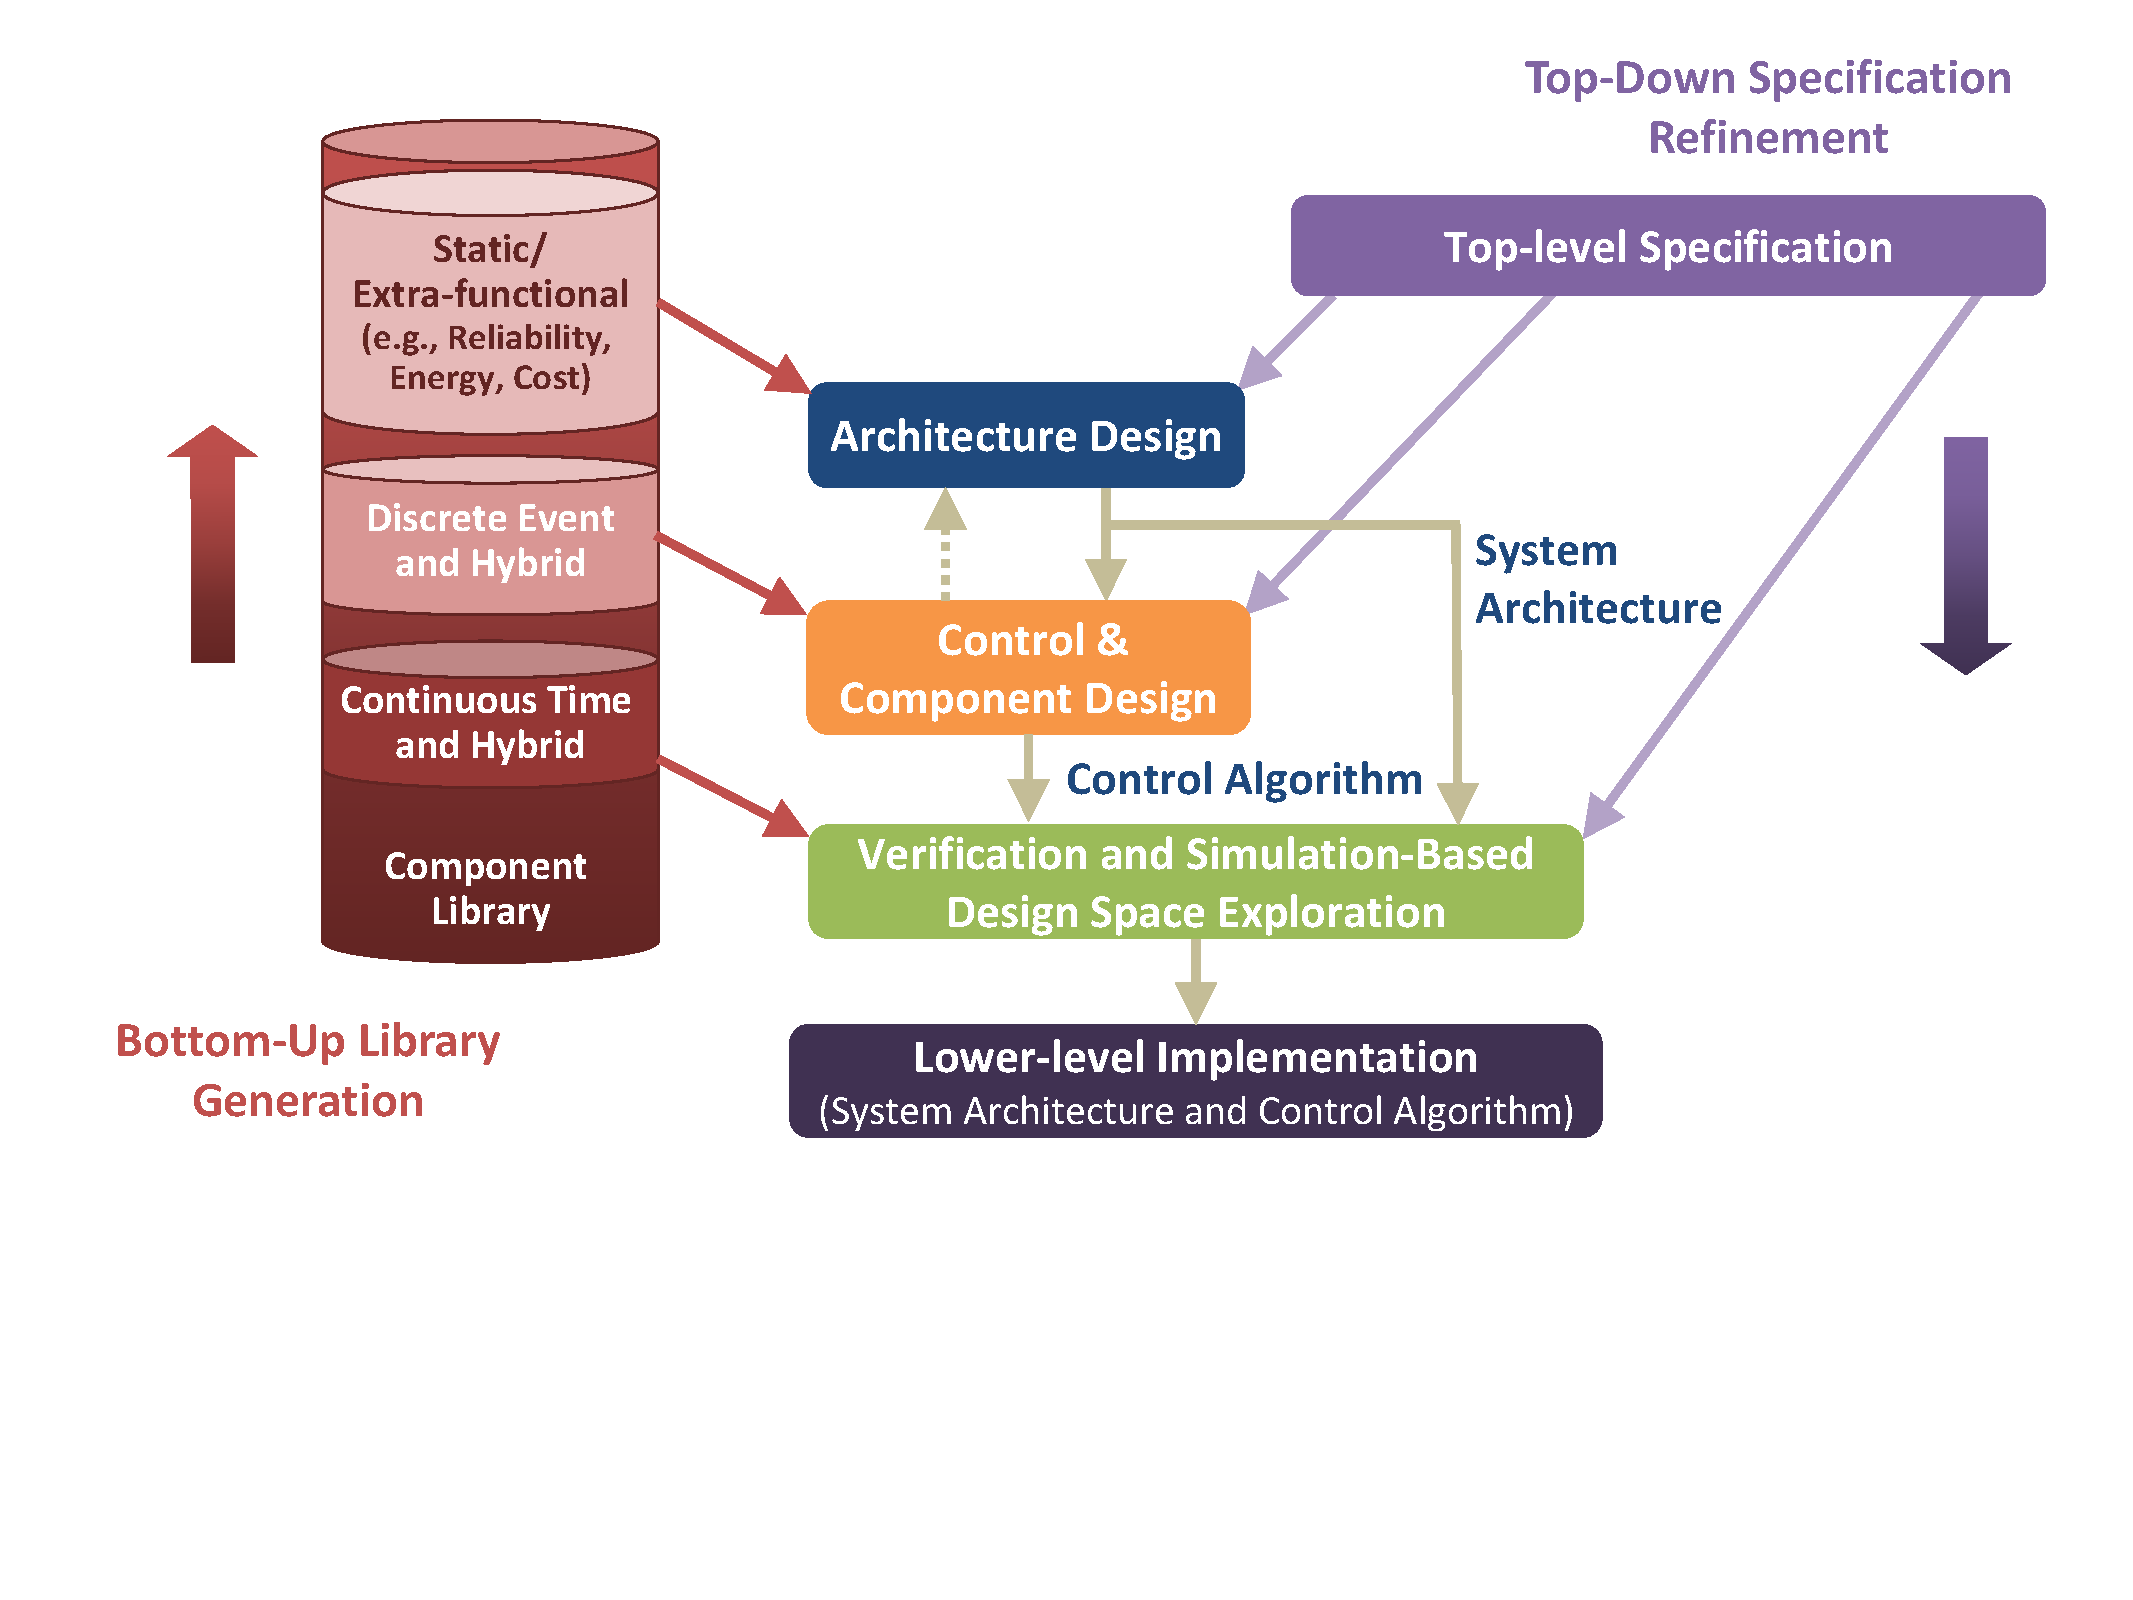
\includegraphics[width=0.6\textwidth,trim={0in 0.15in 0in 0in},clip]{./TA1/structure.pdf}
\vspace{-60pt}
\caption{Structure of the proposed methodology.}
\label{fig:methodology}
\end{center}
\vspace{-25pt}
\end{wrapfigure}

\noindent \textbf{Contracts for LE-CPS Specification, Analysis, and Design.} All the components and their aggregations will be specified by \emph{contracts}, each expressing a set of properties that a component or system satisfies. The contracts will be  used to construct mathematical evidence that a design is correct and consistent with its physical implementation under certain assumptions on the external environment.
% Horizontal contracts will be used to formalize the conditions for correctness of element integration at the same level of abstraction. 
By relying on  contracts, we can provide formal assurance, for instance,  on whether a set of
contracts is realizable, or facets of these are inherently conflicting, and thus no implementation is feasible (contract compatibility or consistency checking).  
% Vertical contracts capture, instead, the conditions for lower levels of abstraction to be consistent with the higher ones, and for abstractions of available components to be faithful representations of the actual parts. 
We will develop algorithms and  tools for capturing requirements of LE-CPSs, for translating them into contracts, for analyzing and validating them using contract operations and relations, and for synthesizing design and verification artifacts from contracts. Recent work from the investigators includes an end-to-end framework for requirement capture, formalization, and validation, which combine a practical front-end formal specification language based on specification patterns together with a rigorous synthesis and verification back-end based on assume-guarantee contracts~\cite{Nuzzo17}. Our framework features a modular and extensible software infrastructure with interfaces that can support different mathematical formalisms as well as pre-existing verification languages and tools. We will significantly extend this framework by developing domain-specific languages for the specification of LE components, systems, and their dynamics as well as supporting automatic translation of requirement patterns to mathematical languages.  Our initial results show that this approach can substantially facilitate the orchestration of formal, exhaustive analyses of temporal properties of CPSs that would otherwise be lengthy, tedious, or error-prone to even formulate, let alone check. 
% Our pattern-based specification language applies to different application domains and hides the details of the requirement formalization, which can be massive, and therefore reduces the chance of errors.

\noindent \underline{\textit{Vertical Contracts for Hierarchical Design.}} 
% The mapping between pairs of models at different abstraction layers can be formalized in several ways. 
% Contracts provide a general semantic framework, but requires definitions in terms of how sets of behaviors are represented and reasoned about. 
We will develop a methodology and scalable algorithms, supported by tools, for hierarchical architecture exploration, mapping between heterogeneous layers, and generation of correctness proofs by combination of formal verification, synthesis, and simulation-based testing techniques. The investigators have demonstrated an approach to hierarchical design on an aircraft power system distribution network~\cite{Nuzzo14,Nuzzo15b}, which combines mathematical optimization tools to reason about  \emph{architecture constraints}, 
% are first formulated as mixed integer linear constraints and 
\emph{linear temporal logic} (LTL)~\cite{pnueli}
% are used to reason about steady-state requirements on system connectivity, cost, performance, and reliability. 
% 
% Additional 
to reason about safety and real-time requirements on a  discrete system abstraction, and 
% by leveraging model checking~\cite{Clark99} and reactive synthesis techniques~\cite{piterman2006synthesis}. Finally, 
signal temporal logic (STL)~\cite{MalerN04} to monitor 
complex dynamical properties related to the physical plant and the hardware and software implementations of the control algorithm by simulation, including   
% contracts on continuous or hybrid dynamical models (continuous abstraction
% in Figure~\ref{fig:methodology}), and monitored  
% % e.g., by leveraging tools such as \textsc{Breach}~\cite{Donze10}. 
% While simulation does not cover, in general, the entire state space, it is sometimes the only computationally feasible choice~\cite{Nuzzo15b}, and can be used, e.g., within 
optimization-based search procedures to approximate unsafe regions of the state space. 
Such a layered approach is a natural framework to explore trade-offs between fidelity of abstractions and scalability of the verification flow. The selection of abstractions and their manipulation was  mostly an \emph{ad~hoc}, manual process, demonstrated on scenario with a dozen requirements on a hybrid model with about $60$ binary and $10$ continuous states without learning components. We contend that orders of magnitude improvements in scalability can be achieved by a systematic, automated, and compositional approach to property-preserving mappings between models. 
% Among the simulation-based tools, we recall 
%    \textsc{Breach}~\cite{Donze10}, a % \textsc{Matlab}/C++ toolbox for the
%    simulation and verification of Signal Temporal Logic properties on systems
%    defined by ordinary differential equations (ODEs) or by external tools, such
%    as \textsc{Simulink}, and \textsc{S-TaLiRo}~\cite{taliro}, another
%    \textsc{Matlab} toolbox for the analysis of continuous and hybrid dynamical
%    systems supporting complex properties in Metric Temporal Logic.
%
% Tools in this
%    category, such as \textsc{UPPAAL}~\cite{uppaal-15years}. \textsc{UPPAAL} can handle models with up to $100$ clock variables, used to capture the continuous dynamics in timed automata.
%
%    \emph{Approximation techniques} can, instead, be used to obtain an answer in
%    some cases, e.g., when dealing with \emph{safety requirements}, which
%    prescribe that ``nothing bad shall happen'' in the design. Among the tools in
%    this category, we recall \textsc{SpaceEx}~\cite{Frehse2011},
%    \textsc{Flow}*~\cite{flowstar}, and \textsc{Ariadne}~\cite{ariadne-lncs2012}.
%    \textsc{SpaceEx} handles systems with piecewise affine, non-deterministic
%    dynamics, while \textsc{Flow}* and \textsc{Ariadne} can also support
%    polynomial and generic non-linear dynamics, respectively. Scalability is,
%    however, limited to a dozen continuous variables for \textsc{Flow}* and
%    \textsc{Ariadne}, while \textsc{SpaceEx} can support up to $100$ variables.
%
% A set of techniques leverage \emph{automatically generated abstractions
%    and refinements} of hybrid models to efficiently answer complex verification
%    tasks. If a finite-state discrete abstraction is not accurate enough to
%    provide a conclusive answer, it is refined until either an answer is found or
%    the maximum number of refinement steps is
%    reached~\cite{Alur2006,ClarkeFHKOST03}.
%    In some cases, the verification problem can be solved with few refinement
%    steps. In this category, we recall \textsc{HybridSAL}~\cite{hybsal}, which
%    handles polynomial hybrid systems with up to $10$ continuous variables, and
%    \textsc{HyCOMP}~\cite{hycomp}, which uses an SMT approach to create discrete,
%    infinite-state abstractions, and was tested successfully on models with up to
%    60 continuous variables with piecewise constant dynamics.
%
% \emph{Automated theorem proving} techniques can also be used to solve
%    verification tasks and perform requirement validation, as in
%    \textsc{KeyMaera}~\cite{Platzer10}, which handles specifications in the
%    temporal logic \textsf{d{\kern-0.1em}$\mathcal{L}$}, and has been
%    successfully used to verify collision avoidance in case studies from train
%    control to air traffic management.
 
We will develop a theory of \emph{vertical contracts} as a foundation to the rigorous and systematic integration of complex systems, to 
fully support  multi-layer design with heterogeneous models, and the generation of correctness proofs by combining effective algorithms and tools at different abstraction layers~\cite{Nuzzo15b}. Intuitively, if vertical contracts are satisfied, a mapping mechanism can be used to produce design refinements that are correct. A formalization of vertical contracts and its systematic implementation to perform model transformations are, however, in their infancy. In model-based verification, abstractions between heterogeneous models were established in the
past for specific pairs of formalisms, such as hybrid abstractions of nonlinear
systems~\cite{Henzinger98,Dang10}, linear hybrid automata abstractions of linear
hybrid systems~\cite{Frehse2008}, discrete abstractions of hybrid systems~\cite{Alur00,Alur2006,Chutinan01}.
Our work will generalize these notions toward a formulation that is compositional and systematically applies to virtually any pair of formalisms.
% To facilitate reasoning at the level of abstraction of requirement engineers, a
% viable strategy is to drive engineers towards capturing requirements in a
% structured form. This can be achieved using a set of predefined high-level
% \emph{primitives}, or patterns, from which formal specifications can be
% automatically generated~\cite{Nuzzo15,Nuzzo15b}. Patterns can also be combined
% together to form higher-level \emph{domain-specific languages} (DSL), as
% exemplified in~\cite{Nuzzo14}. 

\begin{wrapfigure}{R}{0.6\textwidth}
\vspace{-30pt}
\begin{center}
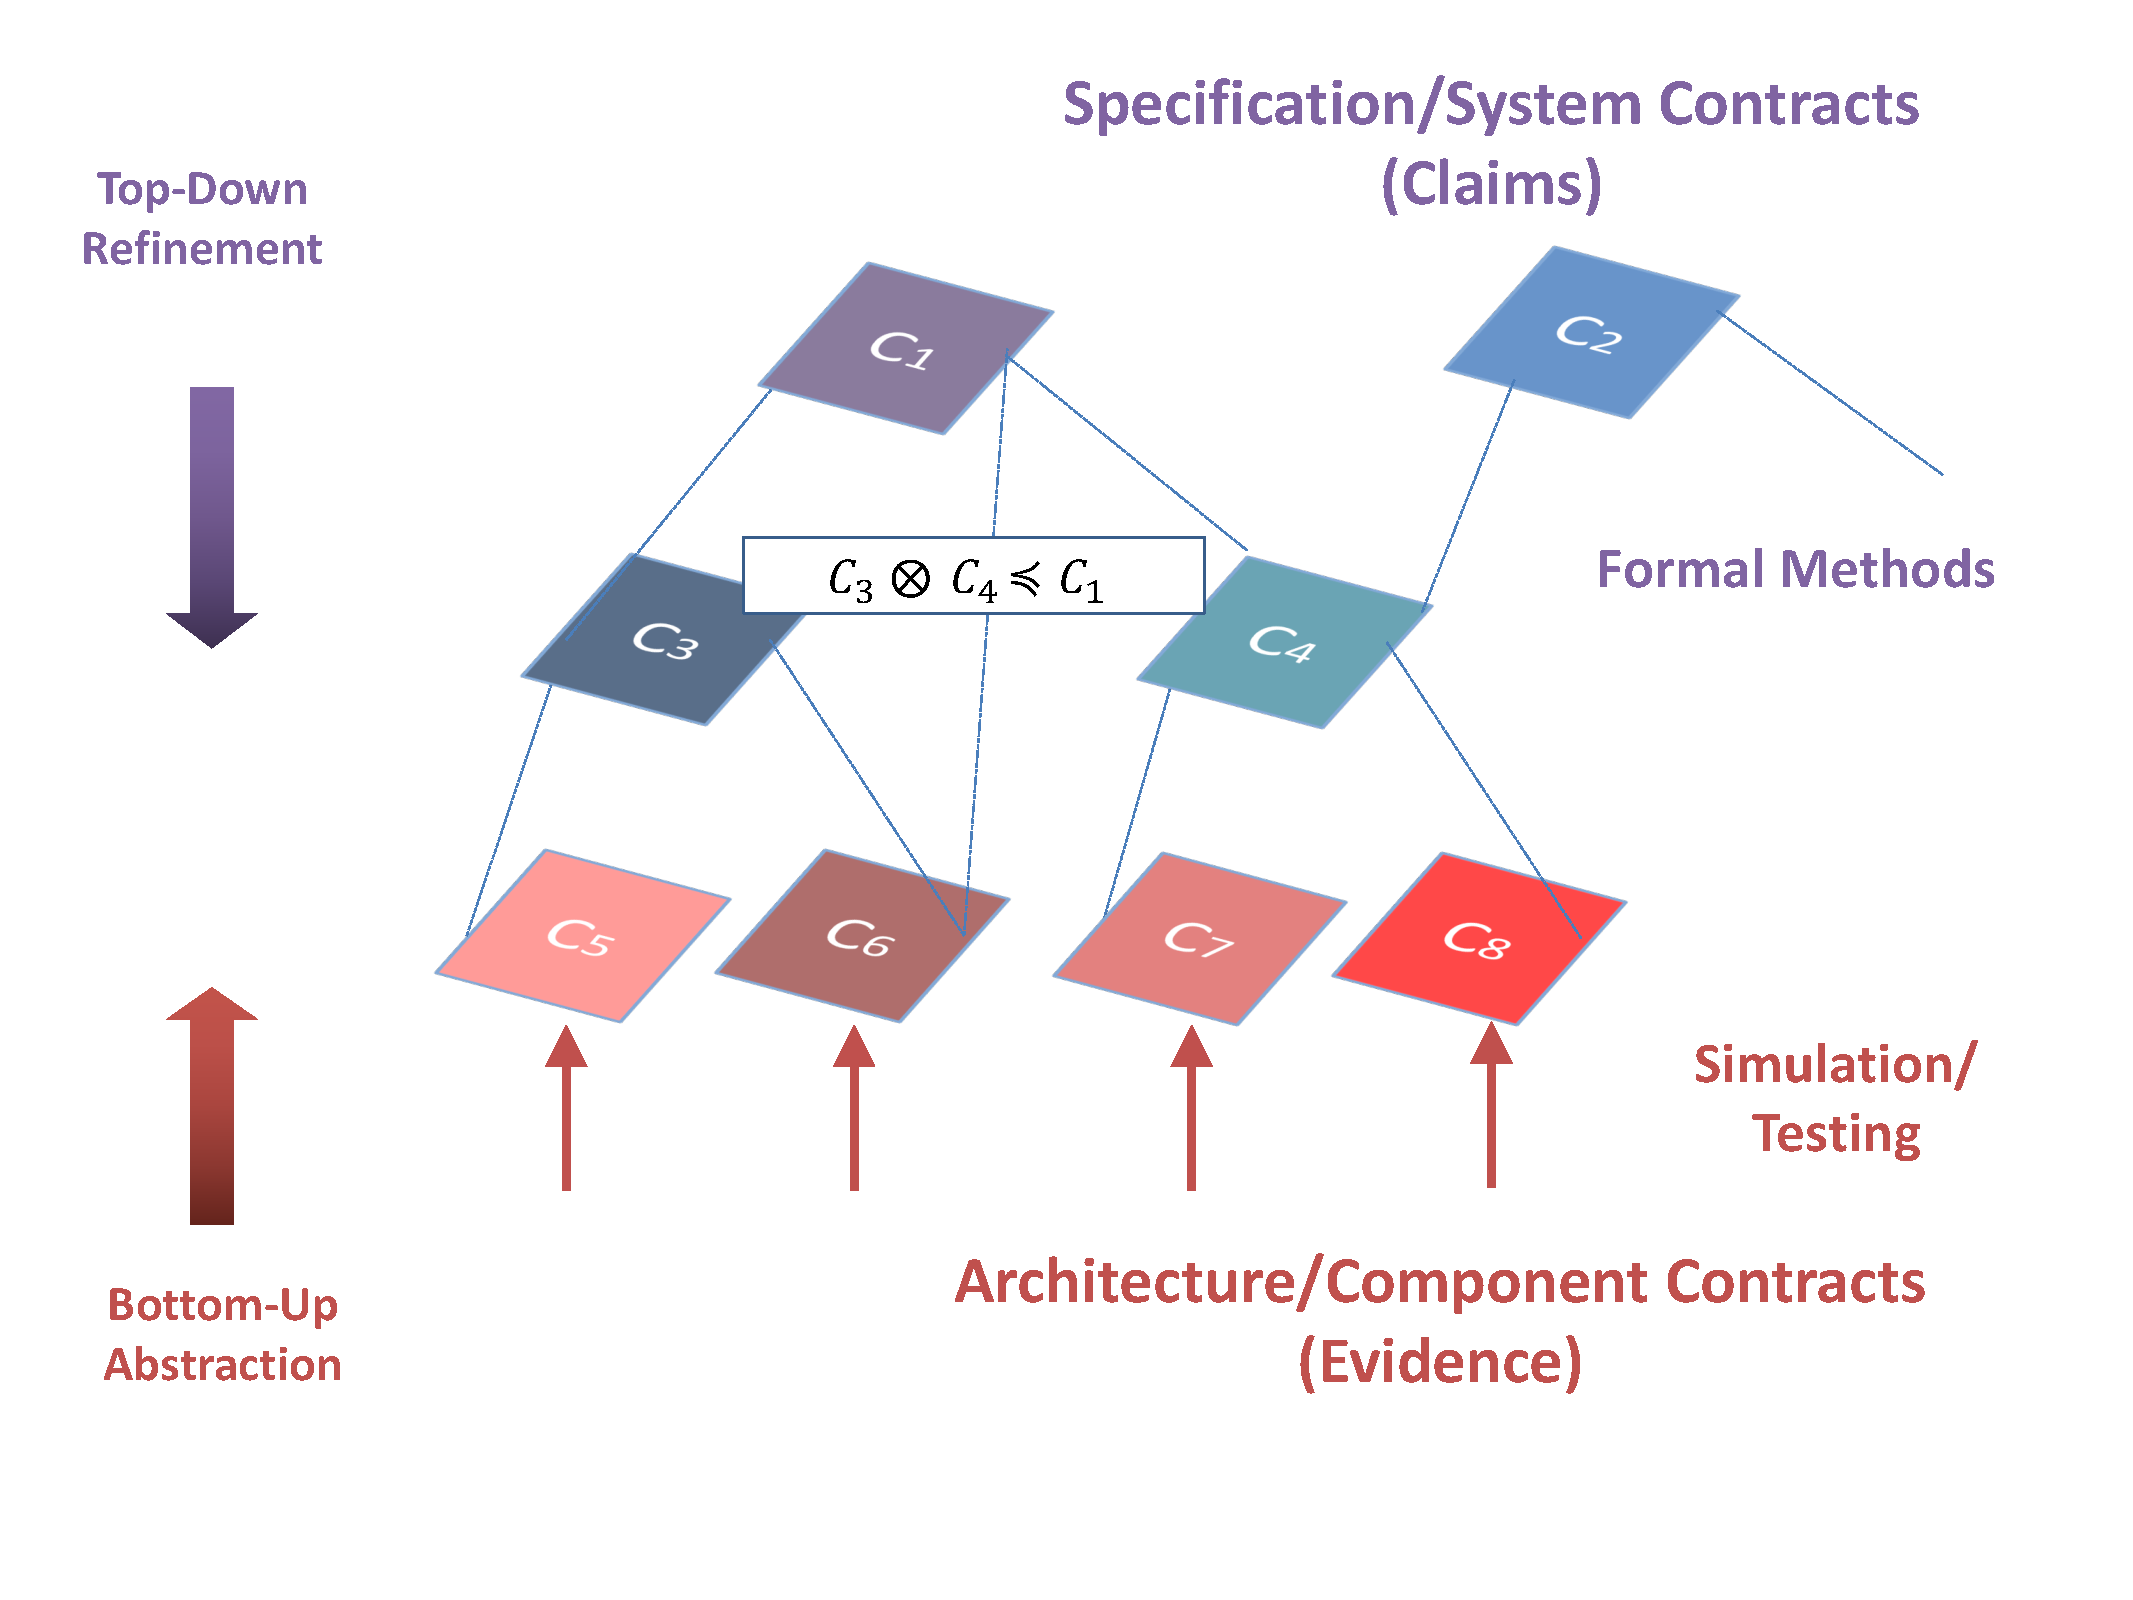
\includegraphics[width=0.6\textwidth,trim={0in 0.15in 0in 0in},clip]{./TA1/Contracts-Assurance-Case.pdf}
\vspace{-30pt}
\caption{Example of contract-based assurance case.}
\label{fig:assurance}
\end{center}
\vspace{-25pt}
\end{wrapfigure}

% Since CPS design
% involves heterogeneous modeling formalisms, each will typically have a
% formulation of the correctness of a refinement or mapping.  
A key criterion on mappings is that they preserve safety properties. 
% that is, if safety property $p$ is established in model $M_1$ and $M_1$ is mapped
% to model $M_2$, then the safety property $p$ holds in $M_2$, without the need to
% reprove it. Refinement mappings between behavioral models are commonly formalized as simulation relations~\cite{Milner89}.  
% The details depend on the
% particular kind of behaviors that a model exhibits, but the essential
% proof obligation is to show that each concrete behavior corresponds in
% a systematic way to some abstract behavior via a simulation relation
% between concrete and abstract states.  Since the behaviors of the
% abstract model are a superset of those required of the implementation,
% then by design the concrete behaviors also satisfy requirements. 
In this program, we will use \emph{abstract interpretation} as a means for verifying and enforcing safety properties in a 
behavioral model. Abstract interpretation works by creating an 
abstraction of the behavioral model in which it is more efficient (1)
to infer state invariants and behavioral properties, and (2) to prove properties on the given model~\cite{Cousot77,Passerone2007}. In this way, we build systematic mechanisms that can encompass any logical breakdown of complex system verification and synthesis problems into arbitrary conjunctive and disjunctive combinations of smaller sub-problems. 
% Moreover, we aim to provide systematic support for richer design refinement relations, including synthesis and optimization based methods, as further detailed below.
% 
% We introduced the notion of vertical contracts to formalize a rich set of design refinement relations for both CPSs~\cite{Nuzzo15b} and analog and mixed-signal systems~\cite{Nuzzo2012,Nuzzo2011}, including refinement via algorithmic synthesis and  optimized mapping of specifications into implementations.  
The resulting verification and synthesis artifacts support the system safety and correctness claim and are returned to the TA3 investigators for the construction of the assurance case. As shown in Figure~\ref{fig:assurance},  lower-level (e.g., physical-level) contracts will mostly be inferred using simulation-based testing to provide conditional evidence for the higher layers. 
% While discrete-time finite-state abstractions are typically preferred, since
% they result into exhaustively analyzable models, the computational complexity of
% analyzing temporal logic contracts for these abstractions can still make
% industrial-scale problems difficult to solve with current tools. There is,
% however, a number of directions to overcome these scalability issues. 
By encapsulating knowledge from feasible implementations of design elements and architectural solutions, a library-based approach spanning different levels of abstraction and granularity will also contribute to reduce the size of the state space and accelerate verification. 
% Contracts will be generated by abstraction of pre-existing designs, or act as virtual components or “placeholders” if an implementation is not yet available.
% In fact, the construction of component models and contracts will be itself driven by our verification or synthesis goals. 
Previous work by the proponents demonstrated up to two orders of magnitude improvement in execution time using a contract library to verify the functionality of embedded controllers subject to architectural constraints~\cite{Iannopollo14}. Similarly, \cite{Finn15} reports about the selection of an optimal aircraft management system design out of a library of over $1.5$M configurations in under two hours, by exploiting simulation-based mapping and a monotonicity property of system requirements with respect to the component library.
% At the lowest level, contracts will be generated from feasible implementations using simulation-based and testing-based approaches. 
% For example, mapping may be cast as an optimization problem where a set of performance metrics and quality factors are optimized over a space constrained by both system requirements and component feasibility constraints. Alternatively, \ldots

\noindent\underline{\textit{Contracts for Probabilistic Reasoning.}} 
% In our scenario, resiliency to unknown environments can be built, for example, using techniques from fault-tolerance design, by leveraging information from multiple sensors, e.g., LIDAR data 
% % to find the objects, 
% and camera data, 
% % to classify the objects.  
% as well as physics-based models to improve on accuracy and safety. 
Learning components are usually required to achieve high accuracy, integrate data from several sensors, and run efficiently on embedded processors. 
% The learning techniques themselves are heterogeneous. % depending on their  architectural structure (hierarchical, decentralized, or centralized), varying environment conditions, and the tight accuracy, latency, and energy constraints. 
In some situations a fast training phase yielding a low-latency, but slightly inaccurate output might be more valuable than a slower but more accurate output. However, such variations in the learning systems must not compromise on key safety and performance objectives. When using machine learning and statistical sensor fusion algorithms to infer information from the external world, providing support for reasoning about probabilistic behaviors and for the development of robust design techniques that avoid over-design becomes crucial. 
% We will develop formalisms and tools for capturing probabilistic requirements and behaviors of LE components, systems, and their dynamics, translating them into contracts for system analysis and design. 
We have recently proposed a contract framework relying on stochastic signal temporal logic (StSTL) to specify and reason about stochastic system behaviors, which is expressive enough to represent hybrid system behaviors and amenable to sound and efficient formulations of verification and control synthesis problems~\cite{Li17}.  We will build on this work to  develop theories and tools for abstraction and analysis of heterogeneous learning systems that can be used to inform architectural decisions and trade performance with computation time.
% Finally, a major challenge for building high-assurance learning systems is to ensure that the accuracy is sufficient to guarantee the safety and performance of the overall system while reducing computation time or power. 
%
% We will provide major innovations by combining learning with formal methods and optimization theory. 
%
% We will develop tools to formally analyze the impact of architectural decisions and multiple design objectives on the safety and performance of learning systems, methods to improve the quality of the training process, and a theory, supported by tools, to guarantee correctness of learning systems with respect to a formal specification.
%
% \pierluigi{\textbf{DOUG/HENNY} \textcolor{red}{[0.75 pages]}:
% \begin{itemize}
% \item brief description on how Kestrel addresses software verification for safety (correctness of low-level software implementations); program analysis? (probably this is not new and we just need to say that we integrate pre-existing technologies with the abstraction and modeling techniques for machine learning components above); 
% \item algorithmic synthesis of monitors. 
% \end{itemize}
% }

% A framework for refinement checking of HRELTL contracts based on SMT solving was
% reported by Cimatti~et~al.~\cite{Cimatti09,Cimatti12}. More recently, we have
% proposed diagnosis and repair algorithms for certain types of STL contracts
% based on the formulation of a set of Mixed Integer Linear Programs (MILPs),
% where infeasibility of a MILP indicates contract in consistencies.
% The proposed algorithms provide feedback on the reasons for unrealizability of
% the STL contracts and suggestions for making them realizable. The resulting
% toolbox \textsc{DiaRY} has been applied to debugging controllers for various
% CPSs, including an autonomous driving application and an aircraft electric power
% system~\cite{ghosh2016}. 

% Finally, in addition to leveraging efficient, off-the-shelf SMT solvers and
% optimization tools, combining the \emph{SMT paradigm} with \emph{optimization
% methods} has recently served as the inspiration for the construction of novel,
% scalable decision procedures and algorithms for cyber-physical system
% verification and
% design~\cite{Nuzzo2010_2,Finn15,Shoukry15,Shoukry15a,Shoukry15b,Shoukry16}.

% \textcolor{blue}{Research challenges:
% \begin{itemize}
% \item  Scalable methods addressing formal verification of safety and liveness properties of LE-CPS;
% \item  Transformations for automated synthesis of assurance monitors.
% \end{itemize}
% }
% We will need to address several scientific challenges to realize our ambitious research agenda. 
% Contract-based design has mostly been applied to systems represented by deterministic models, under pre-defined assumptions and guarantees, prevalently captured using homogeneous formalisms at design time. 
% To support adaptability to changing environments and dynamic reconfiguration, we will need brand-new compositional paradigms that can deal with uncertain behaviors, runtime violations of assumptions or guarantees, and heterogeneous formalisms. 

\noindent\textbf{Scalable Verification and Synthesis via Satisfiability Modulo Convex (SMC) Programming.} 
The robust control of continuous dynamical systems often involves the reduction of the control problem to a convex optimization problem. On the other hand, the design and verification of discrete systems involves the use of Boolean satisfiability (SAT)~\cite{Malik09} solving and related technologies such as satisfiability modulo theories (SMT)~\cite{barrett-smtbookch09}. 
% Since LE-CPSs, neither approach works in isolation as these combine discrete and continuous dynamics. A major challenge is to develop scalable frameworks and computational tools to reason about both domains in tandem. 
% This task will address this problem by substantially extending the emerging satisfiability modulo convex (SMC) optimization framework~\cite{Shoukry2017} they have pioneered to offer such reasoning capabilities. 
Recently, the investigators have devised a new framework that combines both SAT solving and convex optimization, termed as Satisfiability Modulo Convex optimization (SMC)~\cite{Shoukry2017}, that holds great potential for developing efficient computational tools to jointly reason about discrete and continuous dynamics. Preliminary results show that SMC can achieve about 4 orders of magnitude better performance than competing tools on satisfiability problems with a few thousands continuous and Boolean variables. 
% This framework is in its infancy, and we believe it holds great potential for the efficient solution of constraint satisfaction problems as well as the synthesis of control trajectories from contracts in LE-CPSs. 
We will build on this work to develop an SMC toolkit with significantly greater expressiveness, capable of supporting constraint solving problems that arise in the verification and synthesis of LE components and systems in the context of our contract-based approach. Extensions will include support for optimization as well as robust offline and online trajectory planning in the presence of uncertainties. 
% Boolean methods such as SAT solving are effective at reasoning about such combinatorial problems; however, they cannot ignore the vehicle and other system dynamics. Those can be handled through convex programming, but not in isolation – the Boolean constraints interact with the convex constraints. Thus, one needs computational tools to reason about both domains in tandem. The SMC framework offers exactly this combination.

\noindent\textbf{Property Enforcement and Formal Verification by Abstract Interpretation.} 
A system $S$ satisfies a specification $P$ if all behaviors of $S$ are
included in $P$. 
% Given a system description $F:S\mapsto 2^S$ that maps
% states to sets of states, the least fixed point of the predicate
% transformer ${\cal F}(X) = \Theta \vee X \vee F(X)$ starting from
%  $false$ describes exactly the set of reachable states. Thus, for a
% state property $P$ proving satisfaction reduces to proving {\it lfp}$({\cal
%   F}({\it false})) \subseteq P$. 
Proving satisfaction requires the computation of the set of reachable states of $S$, whose termination may be undecidable, or not even guaranteed, in practice. 
% In practice this approach suffers from two
% problems: (1) the sequence ${\cal F}({\it false})$, ${\cal F}^2({\it false})$,
% $\ldots$, may not converge in a finite number of steps, and (2) even
% if it does converge, we may not be able to detect convergence, because the
% inclusion ${\cal F}^{n+1}({\it false}) \subseteq {\cal F}^n({\it false})$ may be
% undecidable.
Abstract interpretation~\cite{Cousot77}, a mathematical theory of approximation
% developed by Cousot and Cousot, 
provides a powerful 
solution to these problem, by performing the computation in an
abstract domain in which the detection of convergence is decidable, and guaranteeing that the results can be translated back to the concrete domain. 
% 
% It performs the forward propagation in an
% abstract domain in which the detection of convergence is decidable,
% resulting in a fixed point that, when translated back to the concrete
% domain, is guaranteed to be a fixed point of the concrete predicate
% transformer. The application of abstract interpretation requires the
% definition of an abstract domain $\Sigma_A$ equipped with a partial
% order $\leq_A$, an abstraction function $\alpha: 2^S \mapsto \Sigma_A$
% that maps sets of concrete states $S \subseteq \Sigma$, into elements
% of the abstract domain, and a concretization function $\gamma:
% \Sigma_A \mapsto 2^S$, 
% such that $\alpha,\gamma$ form a Galois
% connection, that is, they must satisfy $\alpha(S) \leq_A a$ iff $S
% \subseteq \gamma(a)$ for all $S \subseteq \Sigma$ and $a \in \Sigma_A$.
%
The theory of abstract interpretation is well understood and many
abstract domains of various levels of expressiveness have been
proposed in the literature over the past decades~\cite{DBLP:journals/acta/Karr76,DBLP:conf/popl/CousotH78,DBLP:conf/popl/SankaranarayananSM04,DBLP:conf/vmcai/SankaranarayananSM05,DBLP:conf/vmcai/SankaranarayananCSM06}. Its practical
application, however, has proven difficult. Kestrel Technology is one
of only a few organizations that have an abstract interpretation
engine, called CodeHawk, that scales to real-world systems. In particular, CodeHawk has been
applied to sound memory safety analysis of C programs of up to 400,000
lines of code and the analysis of various other (state) properties of
Java programs of more than a million lines of code.

For  behavioral requirements on the CPS, our abstract interpretation technology provides a foundation for the verification of contract refinement relationships described above as well as the generation of efficient, localized monitoring code.
We propose to develop (1) new front ends for our abstract
interpretation engine for the modeling languages created under this
project, that allow proving properties over models and refinements
between different levels of abstractions; (2) new abstract domains
that can express nonlinear behaviors;
(3) a new methodology for proving temporal properties over models and
programs by creating and discharging proof obligations that ensure
system transitions stay within the behavior allowed by an automaton;
(4) a new methodology for enforcing temporal safety properties over
models and programs by refining contracts on components to eliminate
unsafe behaviors;
(5) techniques to provide bounds on performance constraints such as
maximum CPU time and memory usage; and (6) transformations to generate
runtime monitors based on local residual properties that cannot be
proved or enforced.

Conditions to monitor can come from critical assumptions on the CPS design, modeled as automata, and well-known algorithms can be used for synthesizing efficient monitors, e.g., \cite{Havelund04,Rosu08}.
Moreover, in previous work, we explored how to use abstract interpretation to
symbolically simulate a safety property, expressed as an automaton,
over a behavioral model.  This technique can be used to verify that
the safety property holds, and, if a local contract on a component is
too weak to support the property, to refine the contract to eliminate
unsafe behaviors.  Residual conditions from the safety property that
cannot be discharged by verification or refinement are transformed
into runtime monitors and inserted in the code.

% \noindent\textbf{Generation of Runtime Monitors.}
% Conditions to monitor come from two sources: (1) critical assumptions
% on the CPS design and (2) system requirements (including safety
% constraints) that are unproved.  The assumed behaviors of the
% environment can be modeled as automata. There are well-known
% algorithms for synthesizing efficient monitors for automata;
% e.g. \cite{Havelund04,Rosu08}.  Since the environment evolves on its
% own, the monitors depend on sensors to provide relevant events.  For
% behavioral requirements on the CPS, our abstract interpretation
% technology provides a foundation for the generation of efficient,
% localized monitoring code.  The events relevant to a requirements
% monitor arise from the code of the CPS design as it interacts with the
% environment.  By using the abstract interpretation engine to
% symbolically simulate a requirement automaton over the code, we
% annotate the possible safety states that the code could be in.  We use
% transformations to inject any necessary code snippets to
% incrementalize the monitoring and to issue alerts to the TA2 code that
% signal a future violation of the safety constraint.

\noindent\textbf{Simulation-Based Testing and System Testing.}  
During the first phase of the program, we will consider the scenario of an autonomous vehicle moving in an unknown urban environment to prototype our verification methodology and tools. 
% in the presence of other vehicles, and relying on its own sensors for avoiding obstacles, crossing traffic lights, changing lanes, and merging. 
We will then leverage the state-of-the-art microscopic traffic simulator PTV VISSIM to 
% prototype and validate our design flow and 
test the real-time performance and safety of our solutions. VISSIM allows 
simulating traffic patterns based on the dynamics and driver actions of each vehicle as well as their interaction with each other and the road. 
An API allows the user to replace the default driver model  with a customized one as well as implement and simulate the dynamics of learning components in the loop. Further, it allows generating unpredictable scenarios 
% (e.g., incidents,  violations of traffic rules) and generate and 
and collect data to train ML components. As we target industrial-strength platforms, we will also offer a CPS testbed infrastructure that 1) provides a level of fidelity for simulation-based testing that can be relied upon for critical applications and 2) leverages physical model analysis tools to facilitate the identification of problematic behavior spaces. 

\begin{wrapfigure}{R}{0.5\textwidth}
\vspace{-10pt}
\begin{center}
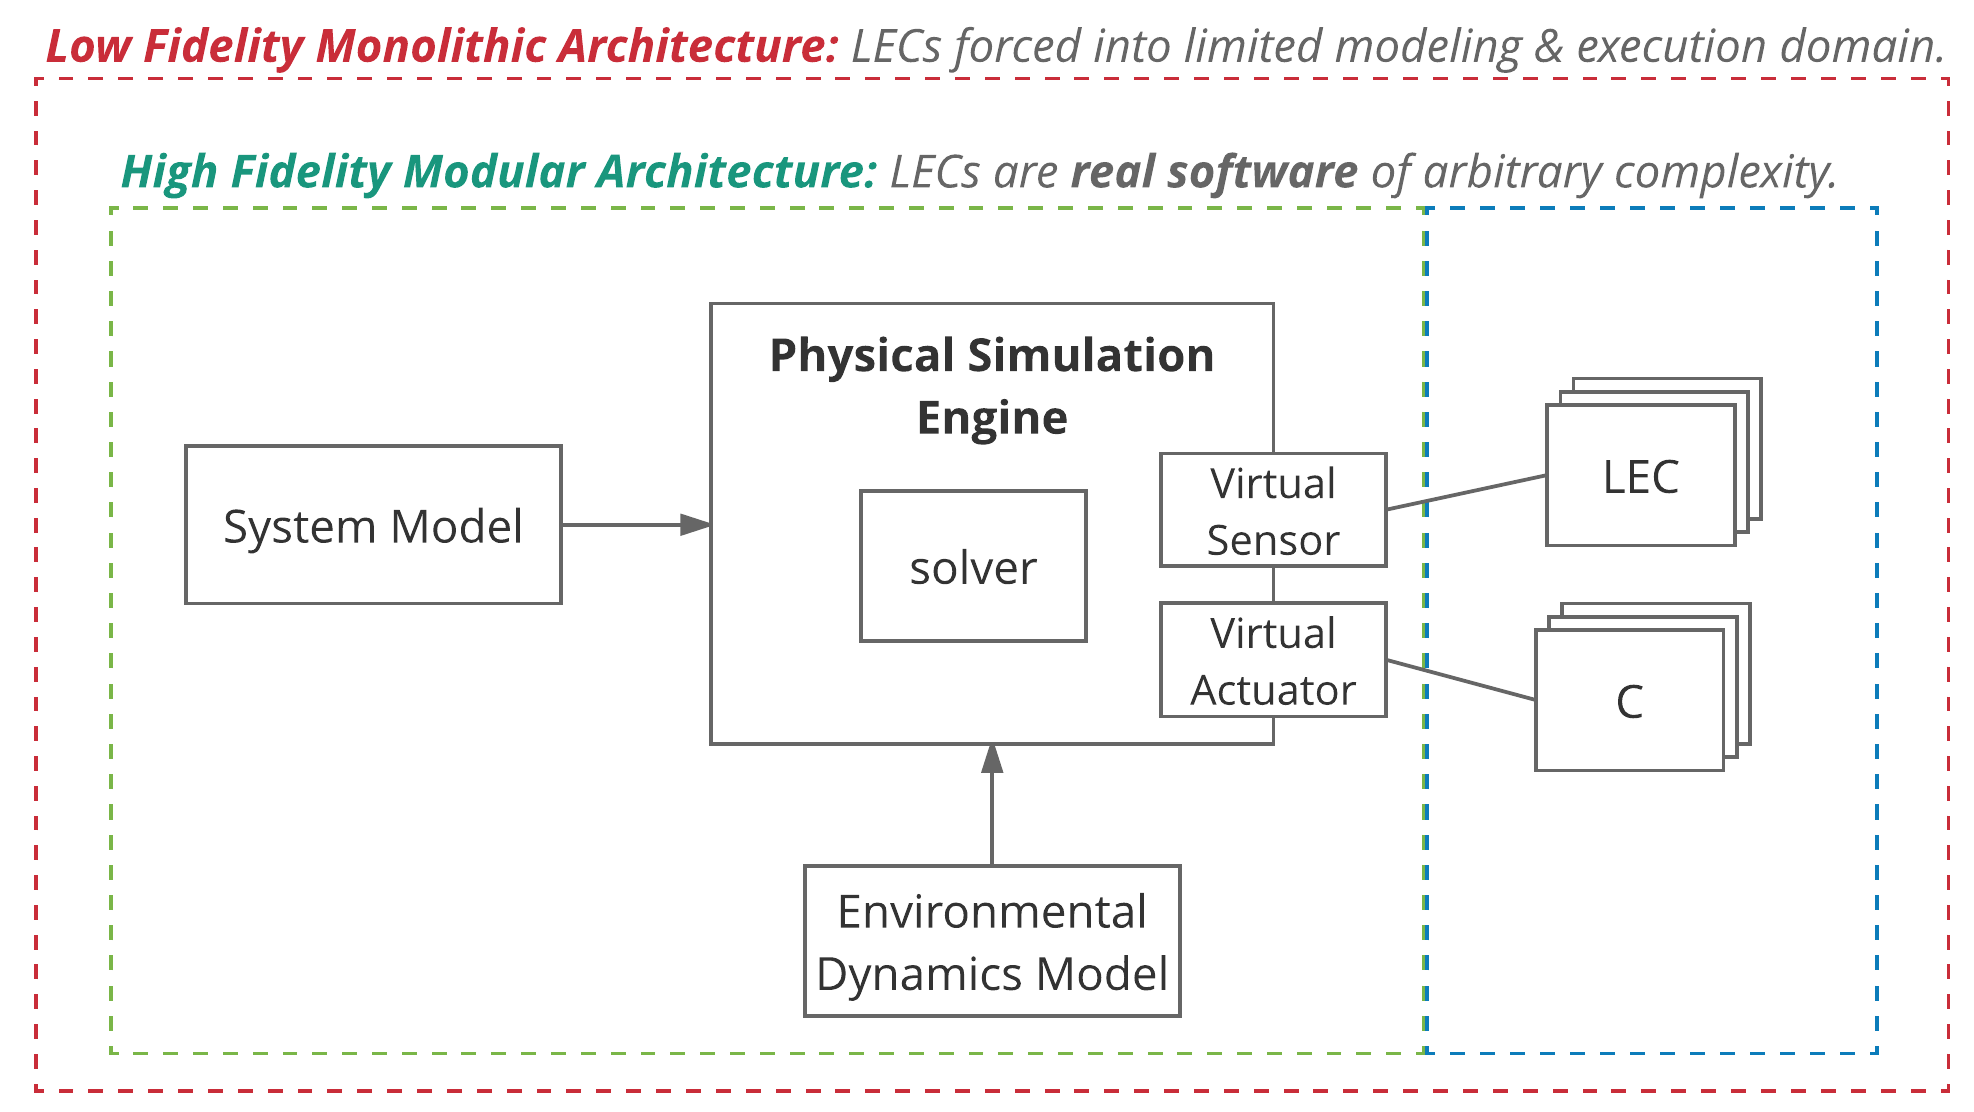
\includegraphics[width=0.5\textwidth,trim={0in 0.15in 0in 0in},clip]{./TA1/simarch.png}
\vspace{-20pt}
\caption{Example of contract-based assurance case.}
\label{fig:arch}
\end{center}
\vspace{-25pt}
\end{wrapfigure}

% \noindent\underline{\textit{High-Fidelity Testbed Environment}}. 
% As shown in Figure~\ref{fig:arch}, 
% shows two possible architectural decompositions of a CPS simulation system. The outer box in red shows a monolithic low-fidelity architecture where the 
Monolithic simulation architectures~\cite{2017OpenModelica,2017WolframAnalysis,2017MapleSimSoftware,2017SimscapeSimulink}, where both the cyber and physical parts of a system are modeled using the same language and executed by a single overarching runtime, provide limited flexibility for industrial-strength designs, since cyber components must be implemented or linked with the language and runtime of the simulation framework.  
% Low-fidelity environments provide a good first order approximation of system behavior, and a rapid development environment as the entire model is developed and executed within a single cohesive program. 
% However, the cyber components must be implemented in the language and runtime of the simulation framework e.g., Simulink subsystems. 
To be able to execute machine learning libraries that could be used in a production setting, in a possibly distributed system\cite{Goodfellow2015Cypress:Systems,Benzel2011TheExperimentation}, we propose, instead, a modular architecture (Figure~\ref{fig:arch}), where  
% The alternative to the monolithic environment is to modularize the simulation architecture into cyber and physical parts. In this architecture 
a physical simulation can interact with cyber components over a network via virtual sensors and actuators. 
% The cyber components can be any software that has the capability of communicating over a network. 
% This means \emph{the software that will go into production can be tested in this environment}. 
We will build on our previous work including a system, called Cypress~ \cite{Goodfellow2015Cypress:Systems}, that follows this architecture and significantly extend it to provide support   
% The following proposed work builds on our previous Cypress work.  %
%Cypress also comes with a holistic CPS modeling language, however, for this program it is anticipated that we will be developing integration software to translate from models that the performers provide into the Cypress underlying representation. As an initial effort in this direction 
% We will provide support 
for the simulation of Modelica models, widely used for modeling DAE-based physical systems. Full Modelica support will be achieved by integrating  parts of the Cypress engine into the OpenModelica engine. 
% The primary engineering integration effort we will undertake as a part of this effort will be the development of time dilation facilities described next.
% \footnote{Some monolithic simulation platforms provide the capability to link to external software, however, the notion of time fidelity is lost and the software in use must be adapted for use with the linking mechanism either directly or through middleware}. 
% The monolithic architecture also loses fidelity, as one cannot test a production software system. 
% For cyber systems that are distributed over a network, the ability to represent the cyber model with any level of accuracy or fidelity is completely lost. 
% The design and implementation of distributed software is notoriously difficult, simulation based testing environments for CPS that can accommodate real distributed systems \cite{Goodfellow2015Cypress:Systems} that integrate with network testbeds \cite{Benzel2011TheExperimentation} are critical on the path to assured systems.
%\subsubsection{Time}
% Solver engines run as fast as they can to achieve a solution at each time step \footnote{save engines that are specifically designed to run in real time, the authors are not aware of any DAE engines that are specifically real time, OpalRT is the closest thing but that engine is squarely in the ODE space}. 
% In the modular architecture, cyber components run asynchronously with respect to the simulator. This may be fine in some situations, but completely invalidating in others. Consider the example of a simulation that runs 100 times slower than real time that is controlled by an external async component. That component has 100x more time than it realistically would to compute a solution, alternatively it could control the simulation 100x more frequently. The problem of a simulation that runs faster than real time is simple, slow the simulation to run in a close approximation of real time. For simulations that cannot keep up with real time, 
To provide timing guarantees, we will pursue a time dilation approach~\cite{Goodfellow2015Cypress:Systems}, where all cyber components run inside virtual machines whose clocks are synchronized to the simulation engine through a protocol that is part of the simulation architecture. Static time dilation mechanisms have been shown to be effective in aligning physical simulation time with the execution time of cyber components~\cite{Gupta2011DieCast}, when a worst case bound on the dilation factor can be computed a priori. We will start with these techniques, and then pursue more recent dynamic time dilation techniques \cite{Lee2014IntegratedDilation}.



%\subsubsection{External Control}
%Cypress already accommodates the mechanical path to external discrete control, by pushing the cyber elements outside the simulation itself and providing a network based interaction mechanism between the cyber and physical. For this effort we will be providing similar mechanisms for external discrete control in OpenModelica, building on the existing OpenModelica device drivers library \cite{Thiele2017TowardsLibrary} for communication.

% \noindent \underline{\textit{Unanticipated Behavior Elicitation \& Test Coverage Maximization}}. 
Many physical systems may be modeled as constrained dynamical systems, represented by DAE, that can be simulated using  
%In the linear setting: $E(t)x(t)^\prime + F(t)x(t) = q(t)$. If $E(t)$ is nonsingular, then it may be factored as $x(t)^\prime = (q(t) - F(t)x(t))E^{-1}(t)$ which is just an ordinary differential equation (ODE). In most situations, however, such a factorization is either not possible or imposes artificial constraints on the causality of dynamics within the system making the model difficult to use in a truly dynamic setting, or reused in different contexts. 
% Because DAE models are natural for many domains and easily generated from CAD tools, research in solvers and analytical methods that operate on DAEs has been quite active since the earliest appearance of CAD tools \cite{Gear1971SimultaneousEquations,Petzold1982ASolver, Brown1994,Marz1992NumericalEquations,Lamour2013,Kunkel2006Differential-AlgebraicSolution,Brenan1995NumericalEquations,Petzold1982Differential/AlgebraicS}. The CAD software community has also started to move from ODE based tools to DAE based as evidenced by 
commercial and open-source tools such as \cite{2017OpenModelica, 2017WolframAnalysis, 2017SimscapeSimulink, 2017MapleSimSoftware, 2017DymolaSimulation}. 
%The most successful solver algorithm that underpins many of the aforementioned is DASSL \cite{Petzold1982ASolver} which is the basis for the very popular open source simulation toolkit Sundials \cite{Hindmarsh2005} from LLNL.
%
%Any system of differential algebraic equations admits a behavior space that may be considered mathematically as a function space. At each time point of integration, the sensitivity of this function space is represented by the underlying Jacobian matrices. For DAEs we typically consider two underlying Jacobians, one for the differential variables and one for the algebraic. Using these matrices, a very simple yet powerful form of behavioral exploration known broadly as sensitvity analysis can be carried out at each integration point as a simulation progresses. Combining physical sensitivity information e.g., what environmental inputs produce disproportionately large changes in variables under observation or control by LE elements, with analytical or qualitative information about the behavior of the LE systems can produce a strategy for test coverage maximization.
% 
Drawing from recent results in the DAE-theory literature~\cite{Berger2013ControllabilitySurvey,Ilchmann2005ATheory,BergerOnSystems,Lamour2013} we will develop a notion of controllability to develop and inform strategies for \emph{unanticipated behavior elicitation and test coverage maximization}. These mechanisms may be viewed as a means to help prune the simulation search space. %
%The precursor to this work goes under the title of \emph{singular control systems} and has been well known since \cite{Dai1989SingularSystems}. However, the work of this era assumes a constant index-1 or lower system, sometimes called a DAE with a regular matrix pencil. %
%More recent work has lifted this constraint 
As the recent work is primarily focused on linear models, we will investigate extensions of these notions to nonlinear models used for LE control systems.  
% so a linearization strategy, possibly similar in spirit to simulation time integration step linearization and exploration must be established. However, this mathematical machinery provides a direct bridge from a system behavioral model into controllability as we understand it today (in multiple contexts, including Kalman and feedback stabilization from autonomous systems) and may provide a similar bridge into LE control systems.

% \begin{wrapfigure}{R}{0.5\textwidth}
% %\vspace{-30pt}
% \begin{center}
% 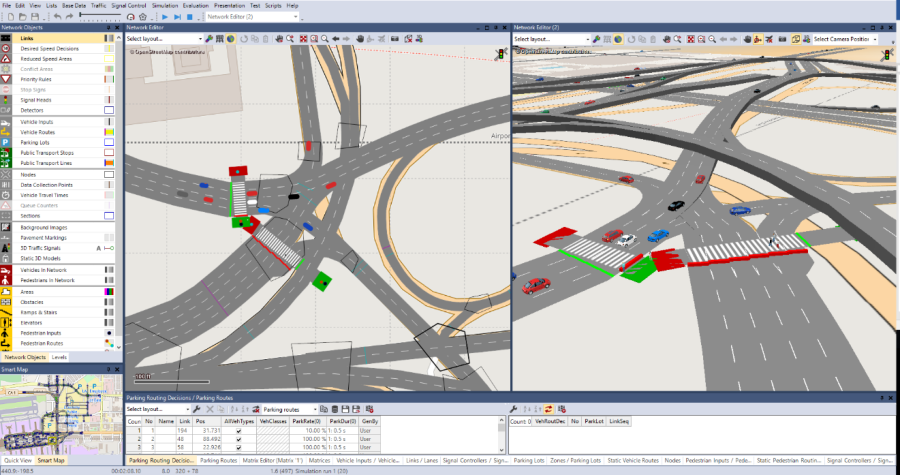
\includegraphics[width=0.5\textwidth,trim={0in 0.15in 0in 0in},clip]{./Simpicture.pdf}
% %\vspace{-30pt}
% \caption{Example of contract-based assurance case.}
% \label{fig:sim}
% \end{center}
% %\vspace{-25pt}
% \end{wrapfigure}

% \noindent \textit{\underline{Vehicle Simulation Platform.}} During the first phase of the program, we will consider the scenario of an autonomous vehicle moving in an unknown urban environment in the presence of other vehicles, and relying on its own sensors for avoiding obstacles, crossing traffic lights, changing lanes, and merging. We will then leverage the state-of-the-art microscopic traffic simulator PTV VISSIM to prototype and validate our design flow and test the real-time performance and safety of our solutions. VISSIM allows 
% simulating traffic patterns based on the dynamics and driver actions of each vehicle as well as their interaction with each other and the road. 
% % It covers motorized private transport, goods transport, rail and road related public transport, as well as pedestrians and cyclists. The simulation software may be used to create detailed computational results or impressive 2D and 3D visualization diagrams. 
% An API allows the user to replace the default driver model  with a customized one. 
% % This new driver model can be applied to part of or to all vehicles in the network.  
% % VISSIM sees the driver model as a black-box, the model is implemented in a DLL that is called once for each vehicle in each iteration of the simulation. 
% Information about the vehicle and its environment is also available for the implementation and simulation of data-driven and online model-based learning algorithms.
% % After processing is done, the driver model must provide a set of outputs that are needed for VISSIM to continue the simulation. Due to this black-box structure the user has a lot of freedom in defining new driver models. The car dynamics and control can be implemented inside the DLL.  As VISSIM gives a certain amount of information about the surrounding vehicles and obstacles, sensors that would measure this information can be easily modeled to the code or stored in external files to be accessed by the DLL during simulation. 
% Among other functionalities, the platform can generate incidents and unpredictable events, introduce different classes of vehicles, and simulate violations of traffic rules at traffic lights. It is then possible to generate and collect data to train ML components in different scenarios.  
% The simulation platform will be used to generate data for the learning enabled components (LEC) in our methodology. F
% For example Gaussian mixture model techniques [1-3] can be used to model how the autonomous vehicle does vehicle following, lane changing, stopping at intersections reacting to obstacles etc. 
% This learning will continue as more data are gathered paying attention to learning unexpected events which once learned and classified can be utilized in future similar cases. 
% This approach has been successfully applied and tested on an actual vehicle in the case of human driving. 

% While VSSIM was successfully used for efficient prototyping of controllers in a human-driving scenario [1-3]. For autonomous vehicles the challenges will be different as sensor inaccuracies in perceiving the environment will affect vehicle actions. In this case earning from past data and relying on them in case of  sensor inaccuracies will be a challenging task that the simulator will help address by generating the data needed under different scenarios.
% Another use of the software platform is to evaluate the real time speed of calculations of certain components of our methodology especially at high speed when actions and decisions have to be made over a much shorter time interval. These tests will allow us to modify or redesign our learning techniques in order to be applicable in real time operations while at the same time guaranteeing safety assurances.  
%Figure~\ref{fig:sim} is screenshot of the simulation of an urban road intersection with auto vehicles, pedestrians and traffic lights. 
% Given our experience with VISSIM and traffic simulations the use of  the road autonomous vehicle as an example operating in a complex urban environment will allow us to generate methodologies that will also apply to surface water vehicles.

% \subsection{Project Plan \textcolor{red}{ALL [0.5 pages]}}
% 
% \textcolor{blue}{\begin{itemize}
% \item Define the project plan - include proposed deliverable and any plans to commercialize/undertake tech transition    
% \end{itemize}}



% Even when a resilient computation, control, and sensing approach can be built using the techniques above, this still needs to be implemented on components such as vehicles, robots, or cloud computing machines. Importantly, the software layers must provide simple programming abstractions to implement the resilient system-level solution by decomposing it into component-level software integrated with protocols for coordination. This task will tackle uncertainty in environments by providing programming abstractions for online environment monitoring, error handling, attack mitigation, and adaptation. 

% To enhance the usability of our tools, we will provide user interfaces based on domain-specific languages that can significantly reduce the burden of formulating exploration problems, raise the level of design capture, and allow automatic translation into mathematical constraints. 

% To devise decompositions and algorithm coordination strategies for design space exploration and mapping, we will build on our previous work on scalable SMT-based decision procedures for a combination of Boolean and convex constraints, an approach we term as satisfiability modulo convex optimization (SMC) [NUZ10, SHO17]. Our initial results already indicate several orders of magnitude improvements in scalability with respect to competing techniques, exclusively based on MILP or SMT. This task will conduct an in-depth investigation of the use of SMC and its extensions to provide support for reasoning about domain-specific constraints and theories specifically tailored to our design and resource management problems. We will develop novel encodings of design space exploration and mapping problems into SMC when accurate compact models are not available in closed form, e.g., when dealing with high-fidelity models of physical plants, stochastic models of networks, cycle-accurate emulators of HW platforms, analog building blocks. We will extend the iterative SMC scheme to rapidly prune the design space and propose candidate configurations, whose performance and cost can be accurately evaluated by simulation. The proposed extension will also deal with models that are trained from data and are not available in analytical form. In the SMC paradigm, providing compact “explanations” of infeasibility, e.g., the minimum number of inconsistent constraints, is key to accelerate the search process by pruning the discrete space. However, finding minimal sets of conflicting constraints is usually expensive. Previous works from our team has investigated efficient schemes to generate infeasibility certificates for convex constraints, and this relies heavily on identifying domain-specific structure. We will develop novel domain-specific methods to generate compact infeasibility certificates tailored to our design problems. These methods will include the application of learning algorithms to infer infeasibility certificates from simulation and verification data.

% For example, the SqueezeDet deep learning based object recognition system seeks to perform object classification for autonomous vehicles quickly at extremely low energy with reasonable accuracy [IAN16, WU16]. But how can one be assured that the accuracy is sufficient to avoid collisions or other unsafe situations? There is a pressing need for techniques for modeling, abstraction, and verification of heterogeneous learning systems.
% This task will develop a new approach to the modeling, abstraction, and verification of heterogeneous learning systems based on the principled combination of formal methods, optimization, and machine learning. It will develop theory and tools to formally analyze the impact of architectural decisions (hierarchy, decentralization, etc.) and multiple design objectives on the safety and performance of learning systems.  

% The accuracy of a learning system depends crucially on the quality of the data set it has been trained on. However, current methods to generate such a data set (e.g., in an active learning framework) mostly ignore the semantics and architecture of the overall system of which the learner is a sub-system. We believe a system-level analysis, guided by a system-level formal specification, can be very effective at generating the right training data for a learning system. For example, [DRE17] shows how system-level counterexamples for an autonomous driving system can be used to generate valuable new training examples for the deep learning based perception component.  Further, we believe the training data must be diverse, with systematic randomized exploration of the feature space.  We will further extend these techniques to online, low-latency algorithms that can improve the training set on the fly during system operation.

% While the above two efforts can substantially improve the accuracy and overall quality of learning systems, they do not guarantee correctness of learning systems with respect to a formal specification. Toward this goal,  when one performs synthesis from examples in safety- and mission-critical systems, one typically needs stronger guarantees of safety and correctness, as captured by a formal specification.  Machine learning algorithms are combined with oracles, typically various computational proof engines, to provide strong correctness guarantees. This task will further develop this nascent theory along with a supporting software toolkit for generating models and controllers for learning systems that must satisfy a formal specification.

% A major challenge in giving formal guarantees for learning systems is to first create a formal model that can be analyzed with computational proof engines. However, learning systems are not static -- they evolve as they encounter new data and new situations. Moreover, modeling a complex machine-learning component such as a deep neural network that has been trained on millions of data points can be challenging enough even if one “freezes” the training process. The verification procedure must account for future changes in the learner as new data arrives. Thus, the first step in this task is to develop techniques to formally model components based on machine learning. We will develop new abstractions for machine learning components and algorithmic techniques to generate those abstract models from implementations. The initial work [DRE17] has shown how even simple approximations of complex learning systems such as deep convolutional neural networks can be effective in finding corner-case bugs and scenarios.
